\documentclass[sigconf,pbalance=true]{acmart}

\usepackage{pgfplots}
\pgfplotsset{compat=1.18}

\setcopyright{none}
\settopmatter{printacmref=false}
\copyrightyear{2026}
\acmYear{2026}
\acmDOI{}
\acmConference[CPSC 8580]{CPSC 8580 Final Project Report}{December 2026}{Clemson, SC}
\acmISBN{}

\begin{document}

\title{CANalyst: Evidence-Linked Explanations for CAN Bus Alerts}

\author{Nicholas DiGennaro}
\email{ndigenn@clemson.edu}
\affiliation{%
  \institution{Clemson University}
  \city{Clemson}
  \state{South Carolina}
  \country{USA}
}

\author{Alexander Salazar}
\email{salaza7@clemson.edu}
\affiliation{%
  \institution{Clemson University}
  \city{Clemson}
  \state{South Carolina}
  \country{USA}
}

\renewcommand{\shortauthors}{DiGennaro and Salazar}

\begin{abstract}
A Controller Area Network (CAN) intrusion detector can flag unusual traffic without explaining the measurements behind an alert. CANalyst packages those measurements and asks a large language model (LLM) to classify the alert and cite evidence for each claim. We evaluate window detection, alert classification, and claim support separately. On a Real ORNL Automotive Dynamometer (ROAD) evaluation partition, a reduced rule profile cuts false positives from 1,461 to 50 across 9,598 negative windows. It detects 910 of 1,954 attack windows, compared with 911 for the original profile. On later Car-Hacking slices, an LLM matches the updated deterministic control at 70 of 70 attack labels after a prompt ablation. On external datasets with vehicle-specific references, the best model labels 34 of 42 selected can-train-and-test attack alerts correctly. Every arm labels 2 of 44 selected TU Eindhoven attack alerts correctly. Two blinded reviewers agree on 32 of 40 sampled claims ($\kappa=0.521$). They both judge 26 supported and six unsupported. These results identify separate limits in detector coverage, label stability, and the support provided by valid citations.
\end{abstract}

\begin{CCSXML}
<ccs2012>
  <concept>
    <concept_id>10002978.10002997.10002999</concept_id>
    <concept_desc>Security and privacy~Intrusion detection systems</concept_desc>
    <concept_significance>500</concept_significance>
  </concept>
</ccs2012>
\end{CCSXML}
\ccsdesc[500]{Security and privacy~Intrusion detection systems}
\keywords{Controller Area Network, intrusion detection, large language models, evidence grounding}

\maketitle

\section{Introduction}

An intrusion detection system (IDS) can tell a vehicle security analyst when traffic departed from a baseline. The analyst still needs to know which measurements changed, which attack labels fit those changes, and where to inspect the underlying frames. CAN makes this difficult because a frame carries an arbitration ID and payload without authenticating the sender. Experiments on production vehicles have documented the security implications of this property~\cite{koscher2010experimental}. Alerts based on rates or timing can help an analyst locate abnormal behavior, but similar measurements can also arise from different attacks or from normal changes in operation.

We built CANalyst to test whether a language model can add useful, checkable context to alerts from a conventional CAN detector. Each model sees a packet of observations from an alert and a local normal reference. It returns a label and claims that cite individual observations. The interface lets an analyst inspect those observations alongside the alert. A deterministic explainer consumes the same packet and provides a comparison that requires no hosted model.

We ask three questions. First, how does reducing the set of alert triggers affect detection and false alarms? Second, how accurate are the attack labels on a fixed set of detected alerts, and how sensitive are those labels to prompt wording and vehicle data? Third, when an explanation cites a valid evidence item, how often do two independent reviewers judge the claim supported?

The main contributions are an implementation that links explanations to measured traffic, controlled comparisons of detector and explainer configurations, and a blinded claim review. The evaluation includes two development datasets and selected traces from two external datasets. Detection and explanation operate on different units of analysis throughout the study. One attack may affect many overlapping windows, and multiple flagged windows may form a single alert.

\section{Background}

\subsection{What a CAN capture reveals}

Electronic control units (ECUs) share a bus and transmit frames with an arbitration ID, data length, and payload. An ID can recur at a regular interval and carry vehicle-specific signals. Raw payload bytes rarely identify a signal's meaning without a separate definition or reverse-engineering work. Repeated values, timing changes, and shifts in payload variation can still provide observables for detection~\cite{marchetti2019read,kulandaivel2019canvas}.

We use attack labels to describe the source datasets and the interpretation an analyst might consider. Denial of service (DoS) can manifest as a shift in traffic concentration or message rate. Fuzzing can create unfamiliar IDs or unexpected payload changes. Fabrication adds frames that may be consistent with spoofing an existing signal. Replay involves previously observed traffic. A similar rate or repeated payload is weak evidence of replay without a sufficiently specific match to earlier traffic. In ROAD masquerade examples, legitimate frames are removed from a fabrication recording. This preserves more of the expected traffic pattern, making the cases difficult for detectors driven by volume or ID novelty~\cite{verma2024road}.

\subsection{Three units of analysis}

A \emph{window} is a short interval scored by the detector. A positive window contains a frame labeled as attack traffic. An \emph{alert} aggregates nearby flagged windows, and its label comes from the attack-labeled frames it contains. An alert with no labeled attack frames is a false alarm for the explainer benchmark. A \emph{claim} is one statement in a saved explanation. A claim can cite an actual packet item and still misread it or draw a conclusion beyond it. Classification accuracy and citation validity therefore answer different questions from claim support.

\section{Related Work}

\textbf{CAN intrusion detection.}
Clock-based IDS (CIDS) uses timing measurements to infer transmitter fingerprints and identify shifts in expected ECU behavior~\cite{cho2016cids}. We use simpler timing summaries to flag windows and preserve observations for review. We do not estimate ECU fingerprints. Song et al.\ use a convolutional neural network to learn sequential CAN patterns~\cite{song2020carhacking}. CAN-BERT learns ID sequences through a masked prediction objective and uses the model for anomaly detection~\cite{alkhatib2022canbert}. CANalyst uses a language model after a detector has already selected an alert. This allows direct comparison with a deterministic explainer on the same inputs.

\textbf{Traffic interpretation.}
READ analyzes bit changes to infer boundaries between signals in raw CAN payloads~\cite{marchetti2019read}. We borrow bit-change summaries as measurements the analyst can inspect. CANvas maps communication relationships between ECUs and message IDs~\cite{kulandaivel2019canvas}. A vehicle-specific map could aid interpretation, but our benchmark packets omit dataset identity and do not assume a verified ECU-to-ID map.

\textbf{Evaluation design.}
Agbaje et al.\ document the difficulty of comparing CAN detectors across experimental settings and propose a common evaluation framework~\cite{agbaje2022framework}. The ROAD dataset documents differences between ambient recordings and the provenance of its masquerade traces~\cite{verma2024road}. Lampe and Meng organize can-train-and-test around known and unknown vehicle and attack combinations~\cite{lampe2024ctt}. We preserve the distinction between reference, tuning, and evaluation inputs within each experiment. The external explanation tests use per-vehicle references and fixed decision logic. They do not measure deployment without a local reference.

\section{System Architecture and Method}

\begin{figure}[t]
  \centering
  \small
  \setlength{\tabcolsep}{5pt}
  \begin{tabular}{@{}rcl@{}}
  Normal reference & $\rightarrow$ & Baseline statistics \\
  Evaluation capture & $\rightarrow$ & Window features \\
  Baseline + features & $\rightarrow$ & Score and merge alerts \\
  Merged alert + frames & $\rightarrow$ & Numbered evidence packet \\
  Same evidence packet & $\rightarrow$ & Rule control or hosted LLM \\
  Label, claims, citations & $\rightarrow$ & Validation and dashboard
  \end{tabular}
  \caption{CANalyst's offline analysis pipeline. The detector uses the normal reference and capture features. The explainer receives only the alert's evidence packet.}
  \Description{Six rows depict normal traffic becoming a baseline and evaluated traffic becoming features. The detector scores and merges alerts. An evidence packet feeds the rule explainer or language model, and output passes to validation and the dashboard.}
  \label{fig:pipeline}
\end{figure}

\subsection{Ingestion, reference, and features}

A Python backend normalizes supported CSV or candump records to timestamps, arbitration IDs, and payload bytes. Evaluation labels stay with the scoring pipeline. Normal reference captures establish expected ID presence, message rates, inter-arrival timing, and payload statistics. The implementation scores 0.5\,s windows at a 0.25\,s stride. Window features include aggregate frame rate, observed IDs, per-ID timing and rate, payload entropy, and bit-change measurements. Empty intervals do not contribute scored windows.

Normal reference coverage matters because a benign drive can contain traffic absent from the reference. For example, different vehicle activity can change the set of transmitted IDs and the distribution of payloads. A window can then exceed a baseline deviation without containing an attack. We compare one ROAD reference recording with seven pooled ambient recordings to measure sensitivity to this choice.

\subsection{Window scoring and alert construction}

The rule detector maps six deviations to scores in $[0,1]$. The components measure aggregate frame rate, unseen IDs, per-ID rate inflation, missing IDs, timing, and payload entropy. Profile v1 takes the maximum of all six. Profile v2 takes the maximum of aggregate rate, unseen IDs, and per-ID rate inflation. Both record all six components for evidence. The fixed decision threshold is 0.55. Profile v2 was selected on tuning captures after missing IDs, timing, and payload entropy produced many alerts on normal traffic and added little attack coverage.

Nearby flagged windows merge into an alert. The merged alert keeps its interval and peak component scores. The evidence builder counts source frames once over that interval. A baseline for each monitored vehicle is necessary because different vehicles can emit different IDs and rates under normal operation.

\subsection{Evidence and explanation}

A packet contains alert boundaries and summary measurements, including frame counts and aggregate rates relative to the reference. It describes salient IDs through counts, rates, timing, and payload statistics. Numbered items such as E0 and E1 give each observation a stable reference. Selected frame samples supply context. Whole-alert and peak-window statistics are labeled separately. Packets omit ground-truth labels, capture names, and dataset identifiers.

The local control applies fixed label rules to the packet. Its revised version uses more evidence for DoS and can label some weak alerts benign. The hosted alternatives receive the same packet and return a predicted label and structured claims linked to evidence IDs. Citation validation verifies that referenced IDs exist. It does not test the meaning of a claim. Strict benchmark replies record errors explicitly so a failed call cannot silently inherit the local control's label.

The React dashboard presents capture timelines, detected alerts, and their supporting data. It links claim citations to packet items and displays saved benchmark runs. The system operates on recorded traffic. Its explanation step does not affect detector thresholds or trigger a vehicle action.

\section{Evaluation}

\subsection{Detection protocols}

The October benchmark established an initial comparison on synthetic traffic, HCRL Car-Hacking~\cite{song2020carhacking}, and ROAD~\cite{verma2024road}. The five-seed synthetic rule detector averaged 0.951 F1, compared with 0.540 for the original IsolationForest configuration. Its aggregate feature set omitted the per-ID jitter-collapse feature available to the rules. It also normalized scores using each evaluated capture, so the comparison reflects the two implementations and their features. The October fixed-rule run scored 42,975 Car-Hacking windows at 0.989 F1 and 6,353 ROAD windows at 0.613 F1. Only 8.1\% of ROAD masquerade windows were flagged. The two normal ROAD holdouts produced one and 378 false positives out of 479 windows each. Those results motivated the reference and profile comparisons.

The November detector benchmark assigns captures or slices to reference, tuning, and evaluation roles. ROAD evaluation contains 20 attack captures and five ambient captures. The scored set has 1,954 positive and 9,598 negative windows. Fabrication captures and their derived masquerade twins stay in the same partition. Four accelerator captures without usable injection intervals are excluded. Car-Hacking uses four attack slices and one normal slice, with 8,616 positive and 13,458 negative windows. Its disjoint reference, tuning, and evaluation slices exclude windows crossing split boundaries.

Car-Hacking supplies frame labels. ROAD labels derive from the published intervals and target IDs, with whole-interval labels for fuzzing. Negative windows include both ambient data and non-attack periods in attack recordings. The reported FPR reflects both sources of negatives. We also inspect ambient-only FPR to see how the detector behaves on drives with no known attack.

We compare fixed profiles at threshold 0.55 and include simple ID and interval baselines, ID entropy, IsolationForest~\cite{liu2008isolation}, and a one-class support vector machine. The unsupervised models fit normal reference data. Tuned thresholds target a 1\% false-positive rate on attack-free tuning windows. We pool confusion counts across evaluation captures. Recall is the fraction of positive windows flagged, precision is the fraction of flags that are positive, and FPR is the fraction of negative windows flagged. Because adjacent windows overlap, the benchmark constructs descriptive 95\% intervals through a block bootstrap of 20-window blocks.

\begin{table}[t]
  \caption{November window detection at threshold 0.55. ROAD has 1,954 positive and 9,598 negative windows. Car-Hacking has 8,616 positive and 13,458 negative windows.}
  \label{tab:detector}
  \small
  \centering
  \begin{tabular}{@{}llrrrr@{}}
  \toprule
  Data & Reference/profile & TP & FP & F1 & FPR \\
  \midrule
  ROAD & Single/v1 & 911 & 1,461 & 0.421 & 15.22\% \\
       & Single/v2 & 910 & 50 & 0.625 & 0.52\% \\
       & Pooled/v1 & 954 & 453 & 0.568 & 4.72\% \\
       & Pooled/v2 & 954 & 50 & 0.645 & 0.52\% \\
  Car-Hacking & Single/v1 & 8,450 & 1 & 0.990 & 0.007\% \\
              & Single/v2 & 8,394 & 0 & 0.987 & 0.00\% \\
  \bottomrule
  \end{tabular}
\end{table}

\subsection{Detection results}

Table~\ref{tab:detector} shows that the reduced profile changes the false-alarm burden on ROAD. With one reference, v2 raises 50 false positives where v1 raises 1,461. The block-bootstrap FPR intervals are $[0.002,0.009]$ for v2 and $[0.126,0.177]$ for v1. Both profiles flag 895 of 971 fabrication and 12 of 12 fuzzing windows. Masquerade recall falls from 4 of 971 windows to 3 of 971. The single-reference v2 precision of 94.8\% therefore coexists with only 46.6\% overall attack recall.

Pooling seven ROAD reference captures cuts v1 false positives from 1,461 to 453. It also helps both profiles detect 44 more fabrication windows. The v2 false-positive count remains 50. The best pooled F1 among the fixed profiles is 0.645 for v2. The pooled whitelist-plus-interval baseline reaches 0.640 with 0.503 recall and 0.014 FPR. These are different operating points. Its extra detections come with more benign flags. Both approaches detect only a small fraction of masquerades. Raising the single-reference v1 threshold through normal tuning removes all flags on this evaluation partition, including all attack flags.

Car-Hacking presents a different trade-off. The reduced profile removes one false positive and misses 56 additional gear-spoofing windows. The whitelist-plus-interval baseline reaches 0.996 F1 with a small increase in FPR. These data do not establish a single detector setting for both datasets. The deployed demo retains v1 while v2 remains an evaluated profile.

The November Car-Hacking v1 rerun returns fewer false positives than the earlier result on the same split (one instead of 32). An isolated rerun attributes the difference to a guard that suppresses jitter-collapse scoring when reference jitter is at or below 10 microseconds. One truncated final line was skipped in the Car-Hacking normal input and the source file was preserved. These implementation details matter when comparing logs across code revisions.

\subsection{Explanation protocols}

Each explanation comparison uses the same frozen alert targets across arms. Scoring uses the majority attack type among labeled frames in each alert. We report correct attack labels over all attack targets, counting failed or missing replies as incorrect. False alarms labeled benign form a separate count. ROAD fabrication maps to spoofing for explanation scoring. The number of labels an explainer can get right depends on how many attacks the detector flagged in the first place.

The original October comparison used 69 Car-Hacking attack alerts and 31 ROAD alerts, including 20 attacks. GLM-5.3 labeled 54 of 69 Car-Hacking and seven of 20 ROAD attacks correctly. The original control labeled 53 and 17 correctly. GLM called 10 of 13 ROAD fabrications replay. Evidence showed that a target ID's message rate roughly doubled. The original wording treated that pattern as characteristic of replay, although fabrication can produce the same observation. An initial evidence packet also undercounted an unseen ID by counting only the first window. We corrected whole-alert counting and added stable citation IDs for alert metadata.

An October follow-up compared revised explainers on the same 100 development targets. The revised control and GLM each got the same 86 of 89 attack labels correct. Qwen3-30B-A3B-Instruct-FP8 got 38 correct. The revision changed both prompt and evidence relative to the first run. Its classification improvement does not estimate an isolated effect of either change.

The October follow-up used a 1,800-token cap, a 90-second timeout, and two concurrent workers per dataset. GLM used low reasoning effort. All 100 replies from each hosted model passed the reference check. Identifier checking still found two explicit IDs absent from GLM's packets. This illustrates a separate validation problem. An existing evidence number can point to the wrong measurement or fail to support an ID mentioned in the surrounding claim.

The November experiments compare Gemma-4-31B, GLM-5.3, and Qwen3.6-27B-FP8 through Clemson's RCD LLM Service. We use whole-alert packets, temperature zero, a 16,000-token cap, and strict replies. The prompt ablation replaces only the DoS description. Later Car-Hacking slices supply 70 attack alerts. Three ROAD ambient captures supply seven false alarms. This set contains no ROAD attack alerts. The separate November rerun of the original 100 targets uses updated packets and prompts. We compare models within each protocol because sharing alert targets does not make the protocols interchangeable.

\begin{table}[t]
  \caption{November later-slice explanation results. Arrows compare prompt v2 with the DoS-wording ablation. Latency is the median over successful replies.}
  \label{tab:heldout}
  \small
  \centering
  \begin{tabular}{@{}lrrrr@{}}
  \toprule
  Arm & Attacks & Benign & Errors & Seconds \\
  \midrule
  Control v1 & $53/70$ & $0/7$ & 0 & $<0.1$ \\
  Control v2 & $70/70$ & $4/7$ & 0 & $<0.1$ \\
  Gemma & $69 \to 70$ & $5 \to 5$ & $0 \to 0$ & $16 \to 19$ \\
  GLM & $59 \to 70$ & $4 \to 4$ & $5 \to 1$ & $36 \to 90$ \\
  Qwen & $37 \to 69$ & $5 \to 5$ & $0 \to 0$ & $55 \to 65$ \\
  \bottomrule
  \end{tabular}
\end{table}

\subsection{Explanation results on development vehicles}

On the later Car-Hacking slices, the updated control gets all 70 labels correct. With the prompt ablation, Gemma and GLM match that count and Qwen gets 69 correct (Table~\ref{tab:heldout}). All six hosted arms correctly classify all 17 DoS targets. The gains come from spoofing predictions. Qwen rises from five to 38 correct among 38 spoofing alerts, while its overall gain is 32 because it loses one fuzzing label. GLM rises from 27 to 38 correct among the spoofing alerts and has fewer reply errors. The DoS wording affected decisions about competing labels.

On the original 100 targets in the November rerun, control v2 gets 85 of 89 attack labels. Prompt v2 Gemma gets 82, GLM 77, and Qwen 50. All four arms miss all four ROAD masquerade cases. Qwen calls 10 of 11 false alarms benign, compared with five for control v2.

On the 69 original Car-Hacking attacks, replacing the DoS wording raises Gemma from 66 to 69 correct, GLM from 61 to 68, and Qwen from 36 to 65. Qwen's correct spoofing labels increase from 5 to 37 of 38. Its correct DoS labels fall from 16 to 15 of 16, and its correct fuzzing labels fall from 15 to 13 of 15. On the same 20 ROAD attacks, Gemma and GLM remain at 16 correct and Qwen rises from 14 to 15. Qwen also loses two correct benign calls. One of GLM's false-alarm replies is missing from the ablation, so a full 11-target benign comparison would require that reply.

Each hosted arm has one recorded run per setting. Median latency includes shared service conditions and varies with the model and prompt. A model that matches control accuracy can still add tens of seconds to a response. Hosted API costs were unavailable. The local control remains a meaningful baseline because it processes the same summary and does not incur these delays.

\subsection{External-vehicle explanation benchmarks}

We evaluated fixed explainers on selected can-train-and-test (CTT) and TU Eindhoven (TUE) traces~\cite{lampe2024ctt,cttdataset,dupont2019tue}. Both benchmarks use local attack-free references for each vehicle. These experiments test previously fixed logic on evidence from other vehicles, with normal reference data available at evaluation time.

CTT uses one reference file per vehicle and 38 scored inputs across four vehicle sets. These include 34 attack files from known-vehicle test splits and four separate normal evaluation slices. The detector produced 196 alerts. We retain all 42 attack alerts and sample 59 of 154 false alarms with a cap of three per capture and a fixed sampling seed. CTT includes 14 DoS alerts, 15 fuzzing alerts, and 13 spoofing alerts. Six of 34 attack files had no detected attack alert. The resulting classification experiment conditions on detector selection.

The TUE experiment uses the Opel Astra and Renault Clio, with reference data from each vehicle's normal training portion. Twelve evaluation inputs include the two benign test logs and ten attack derivatives of those logs. The scope excludes the prototype, and suspension scenarios have no positive frames to label in this protocol. For the edited captures, ground truth comes from comparing with the matched benign log. Diagnostic injection and ID fuzzing map to the fuzzing label. Payload-only edits map to masquerade. Neither payload-edit file produced an alert, and neither benign test log produced an alert. The 44 detected attack alerts comprise 40 fuzzing-family alerts (20 diagnostics and 20 ID fuzzing), two DoS alerts, and two replay alerts. Vehicle attack files from the same original drive share much of their ambient traffic.

\begin{table}[t]
  \caption{External explanation scores on detected alerts. Arrows show prompt v2 and the DoS-wording ablation. CTT benign results use sampled false alarms. TUE contributes zero false-alarm targets.}
  \label{tab:external}
  \small
  \centering
  \begin{tabular}{@{}lrrr@{}}
  \toprule
  Arm & CTT attack (42) & CTT benign (59) & TUE (44) \\
  \midrule
  Control v1 & 28 & 0 & 2 \\
  Control v2 & 29 & 56 & 2 \\
  Gemma & $23\to24$ & $59\to59$ & $2\to2$ \\
  GLM & $31\to31$ & $56\to56$ & $2\to2$ \\
  Qwen & $34\to32$ & $59\to59$ & $2\to2$ \\
  \bottomrule
  \end{tabular}
\end{table}

Table~\ref{tab:external} shows different effects of the prompt change across datasets. On CTT, Qwen prompt v2 gets 34 of 42 correct. Control v2 gets 29. Qwen is correct on nine alerts the control misses and misses four the control gets right. The nine gains are DoS alerts. The four losses include three fuzzing alerts and one spoofing alert (Figure~\ref{fig:ctt-types}). The exact paired McNemar comparison yields $p=0.267$ if alerts are treated as independent. Several alerts share a recording, so this result is descriptive. With the DoS-wording ablation, Qwen falls to 32 correct. Both Qwen settings and both Gemma settings call all 59 sampled false alarms benign. The updated control calls 56 benign. These counts do not give the benign-call rate across all 154 false alarms.

\begin{figure}[t]
  \centering
  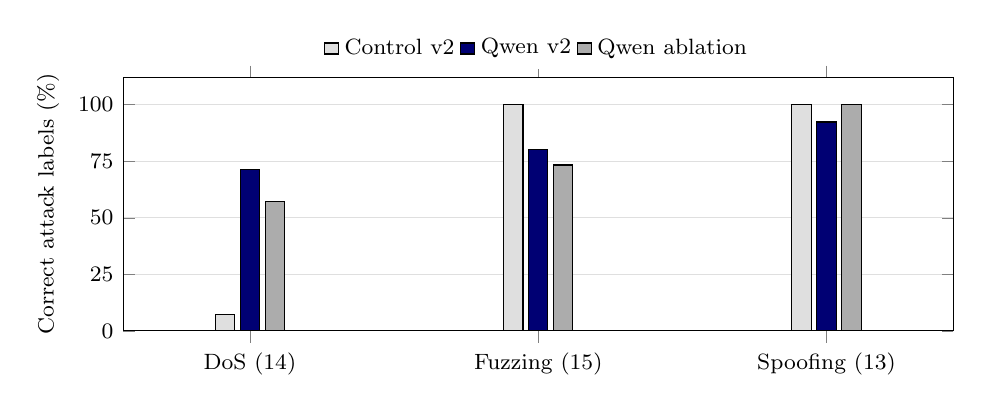
\begin{tikzpicture}
    \begin{axis}[
      ybar, bar width=7pt,
      width=\columnwidth, height=4.8cm,
      ymin=0, ymax=112, ytick={0,25,50,75,100},
      ylabel={Correct attack labels (\%)},
      symbolic x coords={DoS,Fuzzing,Spoofing},
      xtick=data, xticklabels={DoS (14),Fuzzing (15),Spoofing (13)},
      enlarge x limits=0.22,
      tick label style={font=\footnotesize},
      label style={font=\footnotesize},
      ymajorgrids, grid style={gray!25},
      legend style={at={(0.5,1.03)},anchor=south,legend columns=3,font=\footnotesize,draw=none},
      legend image code/.code={\draw[#1] (0cm,-0.07cm) rectangle (0.18cm,0.07cm);}
    ]
      \addplot+[draw=black, fill=gray!25] coordinates {(DoS,7.14) (Fuzzing,100) (Spoofing,100)};
      \addplot+[draw=black, fill=blue!45!black] coordinates {(DoS,71.43) (Fuzzing,80) (Spoofing,92.31)};
      \addplot+[draw=black, fill=gray!65] coordinates {(DoS,57.14) (Fuzzing,73.33) (Spoofing,100)};
      \legend{Control v2,Qwen v2,Qwen ablation}
    \end{axis}
  \end{tikzpicture}
  \caption{CTT label accuracy by attack family among detected alerts. The number of targets for each family appears below its bars.}
  \Description{For DoS, control v2 scores 1 of 14, Qwen v2 scores 10 of 14, and Qwen ablation scores 8 of 14. For fuzzing the three scores are 15, 12, and 11 of 15. For spoofing the scores are 13, 12, and 13 of 13.}
  \label{fig:ctt-types}
\end{figure}

All models and both controls label only the two DoS alerts correctly on TUE. None correctly label any of the 40 fuzzing-family or two replay alerts. A GLM ablation reply is missing, so its recorded coverage is 43 of 44 targets, with two correct.

The identical accuracy scores conceal different errors. Both controls classify 27 of the 40 fuzzing-family alerts as masquerade and 12 as unknown. Gemma calls all 40 benign under both prompts, and the other hosted models also call most of them benign. Neither interpretation matches the label assigned to these edited traces. Sparse ID and diagnostic changes can look weak in a packet dominated by routine traffic. This may explain why the models prefer benign. We did not isolate which measurements or rules caused those decisions.

All eight runs label both replay alerts as spoofing. The evidence includes shifts in observed rates, but it does not establish when identical traffic occurred before the alert. The attack labels in this case come from the paired source logs, not from an independently observed match inside a packet. This is one reason to evaluate what the packet makes identifiable, in addition to scoring the predicted class.

TUE includes a small set of cases derived from two drives. Its failure modes differ from those of CTT, where some hosted models improve on the control for DoS. Neither experiment estimates the overall probability of detecting and naming an attack in external traffic. A complete evaluation needs a target that also counts labeled attack episodes the detector missed.

\subsection{Blinded review of claim support}

Two reviewers independently rated the same 40 claims. We sampled 10 claims each from control v2 and the three hosted prompt-v2 arms on the later-slice corpus. The sampler shuffles claims within ground-truth types and rotates among those types before shuffling the final sheet. That prevents one frequent attack type from filling the sample. A reviewer saw each claim and its cited items with the authoring arm and ground-truth label hidden. The rubric assigned one of three labels. Supported means each factual statement follows from the cited evidence. Unsupported means some statement goes beyond the evidence. Contradicted means cited evidence conflicts with at least one statement. Claims with no citation were outside this review.

\begin{table}[t]
  \caption{Original ratings and outcomes among the 32 agreed claims. Eight disagreements remain unresolved. The agreement row uses the agreed-claim denominator.}
  \label{tab:review}
  \small
  \centering
  \begin{tabular}{@{}lrrrr@{}}
  \toprule
  Ratings & Supported & Unsupported & Contradicted & Total \\
  \midrule
  Reviewer A & 33 & 6 & 1 & 40 \\
  Reviewer B & 26 & 12 & 2 & 40 \\
  Agreed claims & 26 & 6 & 0 & 32 \\
  \bottomrule
  \end{tabular}
\end{table}

The reviewers agreed on 32 of 40 claims (80\%). Cohen's chance-adjusted $\kappa$ is 0.521~\cite{cohen1960agreement}. Of the agreed claims, 26 of 32 are supported and six of 32 are unsupported (Table~\ref{tab:review}). No claim received two contradicted ratings. The reviewers each assigned at least one contradiction, and all of those cases are among the eight disagreements. Excluding disagreement can change the estimated support rate. We report the two original distributions and leave the eight claims open for adjudication.

The agreed sample sizes are unequal. The supported counts are 6 of 8 for control v2, 9 of 9 for Gemma, 4 of 7 for GLM, and 7 of 8 for Qwen. Every arm originally contributes 10 claims. These denominators change when the reviewers disagree, so the agreed subsets can favor easier cases within each arm. Bounds using all 40 claims are also informative: both reviewers support 26 and at least one supports 33. The seven claims between those counts have one supported rating. The eighth disagreement is between unsupported and contradicted.

One agreed unsupported claim described payloads as random. The cited measurements established the share of frames from unfamiliar IDs and the change in bus load. They did not establish how the bytes were generated. One disagreement concerned whether a rise in bus load referred to the busiest window or mistakenly described the whole alert. Both cases show how a valid numerical citation can fail to establish an inference or leave its scope unclear. These ratings measure support in the packet. They do not measure analyst speed, trust, or task completion. The small per-arm sample and unresolved cases preclude a reliable model ranking.

\subsection{Validity and reproducibility}

Car-Hacking influenced rule development. The November detection and explanation sets reuse recordings that were scored in October. The later Car-Hacking explanation slices are temporally distinct from the original explanation slices, but the detector had already evaluated their full sessions. The ROAD evaluation captures have distinct tuning roles in the November detection protocol, but earlier experiments used these recordings. Many ROAD fabrication and masquerade variants also share source traffic. These dependencies limit claims about novel sessions or independent windows.

The external traces broaden vehicle coverage, but each vehicle has a local normal reference. CTT selects a subset of its published files rather than exercising all unknown-vehicle splits. TUE's edited cases share test traffic, and its rare replay class has just two detected examples. Ground-truth mappings compress several source categories into a common label set. The human review samples only one prompt and selected cited claims. It cannot measure whether all explanations capture every important fact.

The experiment archive preserves input hashes, frozen alert packets, run settings, replies, and scores. The local archive audit matched the original file hashes for all 42 CTT and 14 TUE inputs. The original CTT alert-freezing script hash has no matching source in the available repository history. We can verify the saved CTT packets and score their saved replies. Exact regeneration of those packets from the raw captures remains unverified.

The experiment archive under \path{backend/out/} contains the November detector tables, frozen inputs, saved replies, blinded sheets, and original ratings. The build notes in \path{paper/README.md} link to the relevant artifacts. Scoring the saved runs requires no hosted inference.

\section{Conclusion and Future Work}

CANalyst detects abnormal windows, records the evidence behind alerts, and makes generated claims inspectable. Reducing the active rule components lowered ROAD false positives with almost unchanged recall, while most masquerades remained undetected. An updated rule explainer matched or exceeded hosted models on many development comparisons. The prompt ablation improved spoofing classification on later Car-Hacking slices, and the results on CTT and TUE show that those gains did not carry across every corpus. The blinded review found unsupported claims even when the citations resolved to packet items.

Future work should evaluate detector and explainer together on independently collected sessions. It should report how often an attack yields both a detected alert and a correct label. Better temporal or cross-ID features could help detect changes that preserve the normal message rate. Replay classification requires packet evidence that can distinguish prior matching sequences from plausible repetition. A follow-up review should adjudicate the eight claims, sample additional cases across vehicles, and measure whether evidence links improve analyst decisions. These are separate tests of coverage, attribution, and usefulness.

\bibliographystyle{ACM-Reference-Format}
\bibliography{references}

\end{document}
